% -----------
% Copyright 2015, Andrew Lindesay
% Distributed under the terms of the MIT License.
% -----------

\section{Web / Application Server Architecture}

This section covers a broad architectural overview of the system.

\subsection{Elements}

\begin{figure}
\centering
\vspace{.2in}
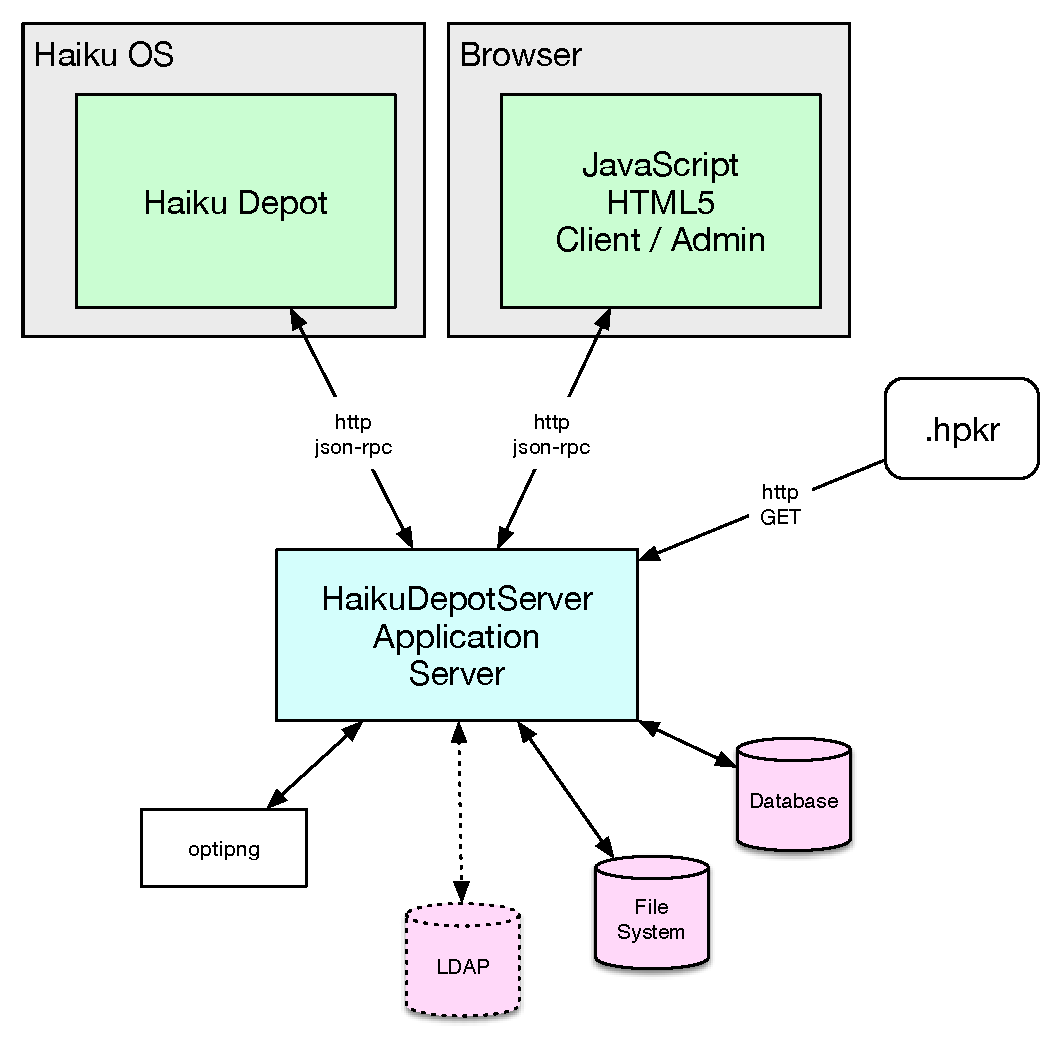
\includegraphics[width=5in]{img-architectureoverview.pdf}
\caption{Overview of the elements of the system.}
\label{\thefigure}
\end{figure}

Figure {\thefigure} shows the elements of the deployed system and how they inter-relate.

The application server is a self-contained java ``jar'' file that contains a packaged-up Tomcat application server container.

The application server communicates (see \ref{api}) with its clients using the HTTP protocol.  The communications are {\it typically} framed as JSON-RPC envelopes, but also straight GET, POST and other requests are employed where appropriate.  The web-front end contains a JavaScript/HTML client that utilizes the same API as is employed by the ``Haiku Depot'' desktop application running on the Haiku operating system.

The application server will, when prompted, import Haiku package repository data from the Haiku package repositories.  To obtain this data it uses HTTP GET requests to obtain the ``.hpkr'' files from each repository.

The application server stores all of its core data in a database.  It also uses local storage for temporary data storage.  The application is able to synchronize its user data with an LDAP database\footnote{Not presently in-use}.

The application server uses the ``optipng'' tool on the deployment host in order to optimize image data.

\subsection{Application Server Infrastructure}

\subsubsection{General}

The application server uses a number of technologies to provide infrastructure for the application server.  The application server is based on java/j2e technology.  It uses the \href{http://projects.spring.io/spring-framework/}{Spring Framework} to manage dependency injection and wiring-up and SpringMVC to manage vending material over HTTP and providing basic HTTP services.  It uses a library called \href{https://github.com/briandilley/jsonrpc4j}{jsonrpc4j} that integrates with SpringMVC to provide JSON-RPC web service APIs.  You can find out more about those APIs in \ref{api}.

\subsubsection{Logging}

The application server uses \href{http://www.slf4j.org/}{SLF4J} to provide for logging.  Other common logging frameworks are re-plumbed into SLF4J in order to centralize logging management.

\subsubsection{Cookies}

The application server does not use HTTP cookies.

\subsubsection{Object-Relational / Data}

The object-relational mapping (ORM) technology used in the project is \href{http://cayenne.apache.org/}{Apache Cayenne}.  Apache Cayenne has a different transaction-handling approach to other common java ORM solutions.  It maintains an in-memory model of the changes made in a context and then flushes those changes to the database when the context is committed.  For this reason, there is no notion of a ``database transaction per request''.  The entities are described in a model file\footnote{There is a desktop-application editor for this model file.} ``cayenne-haikudepotserver.xml'' and the java objects that represent those entities in the running application are in the package ``org.haikuos.haikudepotserver.dataobjects''.  The application server has no formal DAO layer; queries are simply made from the ORM context.  Static methods on concrete entity objects provide easy access to common queries and ``...OrchestrationServices'' beans such as PkgOrchestrationService, UserRatingOrchestrationService and UserOrchestrationService provide more sophisticated functionality in specific domain areas.

Using the Cayenne ``listeners'' such as PostAddCreateAndModifyTimestampListener and UserRatingDerivationTriggerListener the system is able to use changes to entities as a trigger to perform tasks such as update the create and modify timestamp attributes on entities.

\paragraph{Migration}

On first-use the application server will populate the database schema-objects (tables, sequences and so on) itself.  It does this with a library called \href{http://flywaydb.org/}{Flyway}.  Later, as new versions of the application server are deployed, the application server will detect that a database upgrade is required and run the necessary migration scripts.  The migration scripts can be found in the source-code at;

\framebox{\tt /haikudepotserver-webapp/src/main/resources/db/...}

\subsubsection{Multi-Page Web Interface}

The multi-page web interface is designed to provide a simplistic web experience with reduced features for lower-end browsers that have limited JavaScript support.  This interface is public-facing only in that it is not possible to meanigfully authenticate with the system when using the multi-page web interface.  This interface is constructed with the Spring MVC framework and JSP templating.  Pages are rendered server-side and delivered to the web browser.

\subsubsection{Single-Page Web Interface}

The single-page interface is the primary web-based user interface for the system.  It provides functionality directed at public (unauthenticated), authenticated, administrative and root users.  This interface is built using `modern' HTML and JavaScript.  The single-page interface uses the exact {\bf same} APIs as the desktop Haiku Depot application and so is a true client of the application server.

The whole system is treated as ``full stack'' and so the application server as well as the single-page interface are part of the same project and the same build-product.  The application server serves the resources required for the single-page interface.

\paragraph{AngularJS}

The interface is driven by the \href{https://angularjs.org/}{AngularJS} JavaScript framework.  This framework provides for browser-side page rendering, navigational flow.  You can find the AngularJS-centric resources at;

\framebox{\tt /haikudepotserver-webapp/src/main/webapp/js/app/...}

\paragraph{User State}

The ``user state'' including who is authenticated is stored in an AngularJS service within the browser web page.  Because of this and the fact that the single-page interface does not use cookies, refreshing the page will loose the user's authentication and state.  The user's authentication is maintained with the server based on the token.  The token has an expiry and so needs to be periodically refreshed.  Because of this, the user state logic in the client will communicate with the server to refresh the user's token.

\paragraph{Application Localization}

Detail about localization can be found at \ref{applicationlocalization}.

\paragraph{Images}

Where possible, images used in the user interface are provided as SVG so that they can be rendered in a resolution-independent manner.

\paragraph{Delivery}

The single-page interface is delivered by a single JSP page.  The web resources such as the JavaScript files and CSS files are provided by a framework called \href{https://jawr.java.net/}{JAWR}.  JAWR is able to both concatenate as well as compress these resources as they are delivered to the browser.  JavaScript libraries that are used in the project are integrated using \href{http://www.webjars.org/}{WebJars} as maven resources.

\subsubsection{Security}

See \ref{security} for an overview of the authentication and authorization from the perspective of a user.

Although the core Spring Framework is used, Spring Security is not employed in this application server in order to keep the security infrastructure relatively simple.

\paragraph{Authentication}

A servlet filter, AuthenticationFilter exists in the filter-chain in order to intercept any HTTP requests and, where appropriate, to detect an authentication.  If an authentication fails, the filter will not specifically respond; the request will proceed without a user associated with it.  If an authentication is successful then the user is stored in a thread local such that it may be accessed in downstream logic.  Authentication options include both Basic (base 64 username and password pair) as well as a token mechanism.

\paragraph{Authorization}

API exists for answering queries relating to authorization.  The AuthorizationApi endpoint provides these services.  In this way clients are able to check for permissions to undertake operations on some resource.  The types of resources are;

\begin{itemize}
\item Package
\item User
\item Repository
\item User Rating
\end{itemize}

These are typically referenced by their natural or artificial identifier.  In the case of a package this would be the name of the package.  In the case of a user rating, this would be the user rating's code.

Permissions are defined on the ``Permission'' enum.  Examples of permissions include;

\begin{itemize}
\item {\tt REPOSITORY\_EDIT}
\item {\tt USER\_CHANGEPASSWORD}
\item {\tt PKG\_EDITPROMINENCE}
\end{itemize}

The client is expected to hide or show options or data in accordance with a user's security situation, but the application server will also enforce authorization server-side as the client uses API in the system.

Permissions related to packages can be configured in the database on the PermissionUserPkg entity.  Users can be assigned either a specific permission across all packages or for a specific package.

\subsubsection{Email}

Email is delivered with the Spring Framework's email support.  The email templates are produced with the \href{http://freemarker.org/}{Freemarker} library.  The templates for the emails are located at;

\framebox{\tt /haikudepotserver-webapp/src/main/resources/mail/...}

\subsubsection{Jobs}

The application must perform various background jobs from time to time that are impractical to have occur as part of an HTTP request or that are initiated from a process other than an HTTP request.  These are known as ``jobs''.  Examples of situations where jobs are required include;

\begin{itemize}
\item {\tt REPOSITORY\_EDIT}
\item {\tt USER\_CHANGEPASSWORD}
\item {\tt PKG\_EDITPROMINENCE}
\end{itemize}

\begin{figure}
\centering
\vspace{.2in}
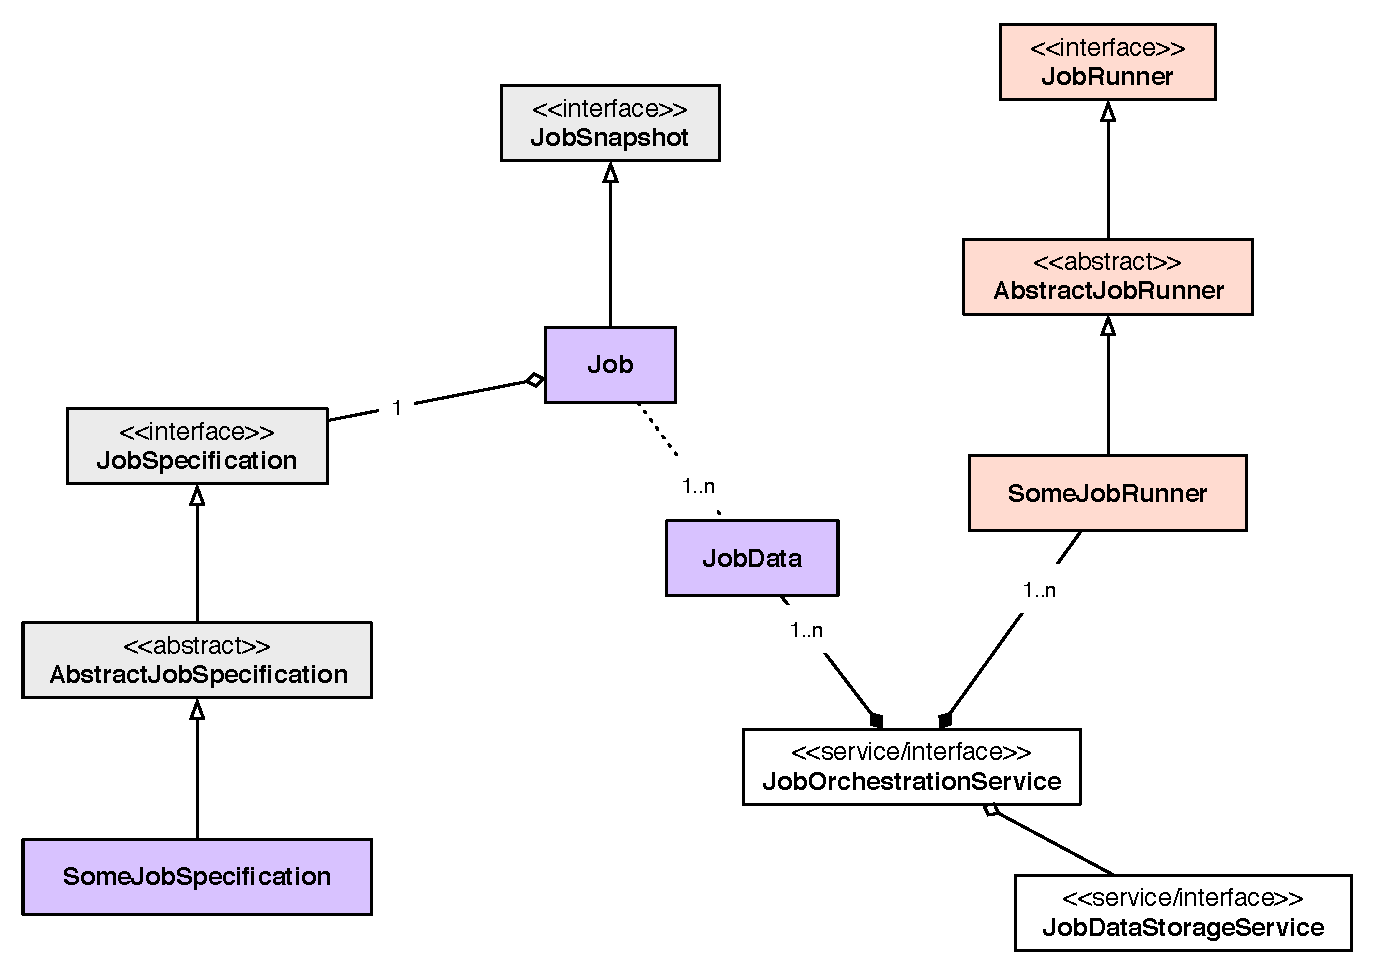
\includegraphics[width=6in]{img-jobsuml.pdf}
\caption{Class-diagram related to the jobs infrastructure.}
\label{\thefigure}
\end{figure}

Figure {\thefigure} shows a number of the key classes that form the functionality of the jobs system.  For each new job, there needs to be an instance of JobRunner and a corresponding instance of JobSpecification.  Together these provide a means of defining the parameters of the job and a means of running the job.

In general, manipulating, enqueueing and querying jobs is done through the JobOrchestrationService.  The service will typically return results of type JobSnapshot.  The JobSnapshot is immutable.  A job is identified by a GUID.  An example of a GUID would be;

\framebox{\tt 98F4B8C0-2F42-4233-813D-AB90C60F6717}

As a job progresses, it moves between a number of states;

\begin{enumerate}
\item {\tt INDETERMINATE}
\item {\tt QUEUED}
\item {\tt STARTED}
\item {\tt FINISHED, FAILED, CANCELLED}
\end{enumerate}

The ``JobSnapshot'' will convey both the state and also the time at which a state transition occurred.

\paragraph{Job Data}

Some jobs require data inputs and outputs.  An example might be a package category import job.  Such a job requires that a spreadsheet of changes is supplied and the job will export a new spreadsheet with a list of the changes made.  This input and output data is managed by the JobOrchestrationService and can be referred to by a GUID.

 The JobSpecification object will maintain a GUID for the suplied input data.  The supplied input data can be populated into the JobOrchestrationService ahead of creating the JobSpecification.

 The JobOrchestrationService keeps track of generated output data and its association with a given job.

\paragraph{Ownership}

The JobSpecification can store a User nickname in order to identify the owner of a job.

\paragraph{Time to Live}

As the application server may be running a number of jobs over time, these would pile-up in the memory of the application server and data related to these reports would pile-up in storage.  To avoid this, jobs have a time-to-live which is specified by the JobSpecification.

\paragraph{Interfacing with Jobs}

API specific to each JobRunner / JobSpecification is provided in order to allow a job to be started from the web interface.

The JobController is able to allow the client to upload supplied input data and for the client to download generated output data via HTTP POST and GET requests respectively.

\subsubsection{Feeds}

The application server is able to produce Atom feeds that can provide updates relating to packages.  The feeds are in the context of one or many packages.  These are produced by the FeedController class which uses the \href{http://rometools.github.io/rome/}{Rome} library to render the feed.

\subsubsection{Captcha}

For some operations such as creating a user or changing password, it is necessary to verify that the user is a human operator and not a machine.  To achieve this, a pictographic representation of a puzzle is shown to the user.  This has a simple textual response.  A mechanism for this is in the "org.haikudepotserver.captcha" package.

A typical use pattern will involve the client first creating a captcha.  This creation process will yield a token for the captcha as well as an image to display to the human operator.  When the second API is used that requires the captcha response, the client's call will contain both the textual response from the human operator as well as the token to identify the captcha.
